\documentclass[14pt,t,usenames,dvipsnames]{beamer}
\usepackage[english]{babel}
\usepackage[misc]{ifsym}
\usepackage{fontspec,mathabx,multicol,listings,comment}
\usepackage{TeXnicalities}
\usetikzlibrary{shapes}

\setsansfont{Yanone Kaffeesatz}[
    UprightFont     = *-Regular ,
    BoldFont        = *-Bold ,
    BoldItalicFont  = *-Bold ,
    BoldSlantedFont = *-Bold ,
    ItalicFont      = *-Light ,
    SlantedFont     = *-Light ,
    SmallCapsFont   = *-Thin
]

\graphicspath{{Figures/}}
\usepackage{listings}
\def\transpPerc{100}
%listings set
\lstdefinestyle{MyCpp}{
% backgroundcolor=\color{white},    % choose the background color; you must add \usepackage{color} or \usepackage{xcolor}
breakatwhitespace=false,            % sets if automatic breaks should only happen at whitespace
breaklines=true,                    % sets automatic line breaking
captionpos=b,                       % sets the caption-position to bottom
deletekeywords={...},               % if you want to delete keywords from the given language
escapeinside={@|}{|@},                % if you want to add LaTeX within your code
extendedchars=true,                 % lets you use non-ASCII characters; for 8-bits encodings only,
                                    % does not work with UTF-8
frame=none  ,                       % adds a frame around the code
numbers=none,                       % where to put the line-numbers; possible values are (none, left, right)
numbersep=5pt,                      % how far the line-numbers are from the code
numberstyle=\tiny\color{black},     % the style that is used for the line-numbers
rulecolor=\color{black},            % if not set, the frame-color may be changed on line-breaks within not-black text
                                    % (e.g. comments (green here))
showspaces=false,                   % show spaces everywhere adding particular underscores; it overrides 'showstringspaces'
showstringspaces=false,             % underline spaces within strings only
showtabs=false,                     % show tabs within strings adding particular underscores
stepnumber=2,                       % the step between two line-numbers. If it's 1, each line will be numbered
stringstyle=\color{OliveGreen},     % string literal style
tabsize=2,                          % sets default tabsize to 2 spaces
title=\lstname,                     % show the filename of files included with \lstinputlisting; also try caption instead of title
%
%Base style for this presentation 
keepspaces=true,                    % keeps spaces in text, useful for keeping indentation of code
                                    % (possibly needs columns=flexible)
keywordstyle=\color{Cyan},          % keyword style
language=C++,
basicstyle=\ttfamily\scriptsize\color{black},
keywordstyle=\color{OliveGreen},
stringstyle=\color{Magenta},
commentstyle=\color{red},
moredelim=[is][\color{ForestGreen}]{|+}{+|},
literate=% literate={<replace>}{<replacement text>}{<width>}
  {\#define}{{{\color{CarnationPink}\#define}}}{6}
  {\#include}{{{\color{CarnationPink}\#include}}}{7},
morekeywords={real, vector, Minesweeper, myVecVec, Cell, SetOfCells, regex, T, string, CD,
              invalid_argument, Jukebox, Coffee, Version, Point2D, Point3D, Person, pair},
emph=[1]{calculateAverage, size, exit, begin, end, find, makeReportForUser, isElementInVector,
         main, WelcomeUserToTheGame, playGame, PrintGameResult, isPrime, sqrt, push_back, FC,
         getFlaggedCells, isFlagged, at, isEligibleForFullBenefits, gsl_fcmp, getDefaultForHelper,
         trim_right, addCD, MakeCoffee, WarmUpMachineIfNeeded, GrindCoffee, SetPressureAndTemperature,
         BrewCoffee, getMajorVersionNumber, getMinorVersionNumber, getBuildNumber, Distance, factorial,
         Q_rsqrt, Q_fastInverseSqrt, calculateApproximateInverseSqrt, refineResult, get, fetch, retrieve, obtain},
emphstyle=[1]{\color{NavyBlue}}, %Functions
emph=[2]{cout, data, sum, sum1, sum2, data, dataSet, dataSet1, dataSet2, first, last, argc, argv, minesweeper,
         number, i, c, f, b, list, gameBoard, flaggedCells, cell, realDaysPerIdealWeek, totalRealWeeksNeeded,
         realDaysPerTask, taskDaysEstimate, realWeeksPerTask, j, e, employee, timePattern, iterationNumber,
         functionValue, epsilon, it, value, keyToDecipher, longTitle, longAuthor, durationInMinutes, cd,
         typeOfCoffee, x, y, z, x2, approximateResult, floatAsInteger, initialNumber, refinedResult,
         threehalfs, result, timestamp, ymdhms},
emphstyle=[2]{\color{Orange}}, %Variables
emph=[3]{if, else, while, do, for, case, switch},
emphstyle=[3]{\color{violet}}, %Loops, if, etc.
emph=[4]{const, auto, break, continue, default, static, return, struct, NULL, sizeof, typedef,
         template, typename, true, false, throw, public, class},
emphstyle=[4]{\color{ProcessBlue}}, %Logical keywords
emph=[5]{std, boost},
emphstyle=[5]{\color{Maroon}}, %Namespaces
emph=[6]{STATUS_VALUE, FLAGGED, WORKING_DAYS_PER_WEEK, NUMBER_OF_TASKS, HOURLY_FLAG,
         CG_CHECK_RESIDUUM_EVERY, BOOST_AUTO_TEST_CASE, BOOST_TEST_MODULE, BOOST_REQUIRE_EQUAL},
emphstyle=[6]{\color{Gray}}, %Macros
emph=[7]{age, flags, title, author, tracks, duration, cdList},
emphstyle=[7]{\color{Peach!50!Purple}}, %Members
emph=[8]{Factorial, SpecialCases, NormalCases},
emphstyle=[8]{\color{Blue}}, %Boost cases and suite
}


\def\CPP{\lstinline[style=MyCpp, basicstyle=\ttfamily\color{black}]}

\makeatletter
\newenvironment{CenteredBox}{% 
\begin{Sbox}}{% Save the content in a box
\end{Sbox}\centerline{\parbox{\wd\@Sbox}{\TheSbox}}}% And output it centered
\makeatother


\usetikzlibrary{fadings}

\pgfkeys{%
/piechartthreed/.cd,
scale/.code                =  {\def\piechartthreedscale{#1}},
mix color/.code            =  {\def\piechartthreedmixcolor{#1}},
background color/.code     =  {\def\piechartthreedbackcolor{#1}},
name/.code                 =  {\def\piechartthreedname{#1}}}

\newcommand\piechartthreed[2][]{% 
   \pgfkeys{/piechartthreed/.cd,
     scale            = 1,
     mix color        = white,
     background color = white,
     name             = pc} 
  \pgfqkeys{/piechartthreed}{#1}
  \begin{scope}[scale=\piechartthreedscale] 
  \begin{scope}[xscale=5,yscale=3] 
     \path[preaction={fill=black,opacity=.8,
         path fading=circle with fuzzy edge 20 percent,
         transform canvas={yshift=-15mm*\piechartthreedscale}}] (0,0) circle (1cm);
    \fill[gray](0,0) circle (0.5cm);  
     \path[preaction={fill=\piechartthreedbackcolor,opacity=.8,
          path fading=circle with fuzzy edge 20 percent,
          transform canvas={yshift=-10mm*\piechartthreedscale}}] (0,0) circle (0.5cm);
     \pgfmathsetmacro\totan{0} 
     \global\let\totan\totan 
     \pgfmathsetmacro\bottoman{180} \global\let\bottoman\bottoman 
     \pgfmathsetmacro\toptoman{0}   \global\let\toptoman\toptoman 
     \begin{scope}[draw=black,thin]
     \foreach \an/\col [count=\xi] in {#2}{%
     \def\space{ } 
        \coordinate (\piechartthreedname\space\xi) at (\totan+\an/2:0.75cm); 
        \ifdim 180pt>\totan pt 
         \ifdim 0pt=\toptoman pt
            \shadedraw[left color=\col!50!\piechartthreedmixcolor,
                       right color=\col!25!\piechartthreedmixcolor,
                       draw=black,very thin] (0:.5cm) -- ++(0,-3mm) arc (0:\totan+\an:.5cm) 
                                                       -- ++(0,3mm)  arc (\totan+\an:0:.5cm);
            \pgfmathsetmacro\toptoman{180} 
            \global\let\toptoman\toptoman         
            \else
            \shadedraw[left color=\col!50!\piechartthreedmixcolor,
                       right color=\col!25!\piechartthreedmixcolor,
                       draw=black,very thin](\totan:.5cm)-- ++(0,-3mm) arc(\totan:\totan+\an:.5cm)
                                                        -- ++(0,3mm)  arc(\totan+\an:\totan:.5cm); 
          \fi
        \fi   
        \fill[\col,draw=black] (\totan:0.5cm)--(\totan:1cm)  arc(\totan:\totan+\an:1cm)
                                     --(\totan+\an:0.5cm) arc(\totan+\an:\totan :0.5cm);     
       \pgfmathsetmacro\finan{\totan+\an}
       \ifdim 180pt<\finan pt 
         \ifdim 180pt=\bottoman pt
            \shadedraw[left color=\col!50!\piechartthreedmixcolor,
                       right color=\col!25!\piechartthreedmixcolor,
                       draw=black,very thin] (180:1cm) -- ++(0,-3mm) arc (180:\totan+\an:1cm) 
                                                       -- ++(0,3mm)  arc (\totan+\an:180:1cm);
            \pgfmathsetmacro\bottoman{0}
            \global\let\bottoman\bottoman
            \else
            \shadedraw[left color=\col!50!\piechartthreedmixcolor,
                       right color=\col!25!\piechartthreedmixcolor,
                       draw=black,very thin](\totan:1cm)-- ++(0,-3mm) arc(\totan:\totan+\an:1cm)
                                                        -- ++(0,3mm)  arc(\totan+\an:\totan:1cm); 
          \fi
        \fi
        \pgfmathsetmacro\totan{\totan+\an}  \global\let\totan\totan 
       } 
    \end{scope}
    \draw[thin,black](0,0) circle (0.5cm);
   \end{scope}  
\end{scope}
}



%Tikz
\tikzset{
    %Hexagons
    hexagon/.style n args={3}{double arrow, double arrow head extend=0cm, inner sep=3pt, draw=#1, fill=#2, text=#3, thick},
    hexagon/.default={black}{gray!20}{black},
    hexagonOne/.style={hexagon={#1}{#1!30}{#1}},
    hexagonTwo/.style 2 args={hexagon={#1}{#1!#2}{#1}},
    hexagonThree/.style n args={3}{hexagon={#1}{#1!#2}{#3}},
    hexagonShade/.style n args={3}{double arrow, double arrow head extend=0cm, inner sep=3pt, thick, draw=#1, left color=#2, right color=#3},
    %General text element
    Shape/.style n args={3}{draw=#1, fill=#2, text=#3},
    genShape/.style 2 args={#1, inner sep=3pt, draw=#2, fill=#2!20, text=#2, thick},
    halo/.style={preaction={draw, #1, line width=7, -}},
}

%My commands
\newcommand<>{\tc}[2]{\textcolor#3{#1}{#2}}
\lstnewenvironment{Cpp}[1][]
    {\lstset{style=MyCpp, belowskip=-7mm, aboveskip=0pt,#1}}
    {}


\makeatletter
\patchcmd{\beamer@sectionintoc}
  {\vfill}
  {\vskip2ex}
  {}
  {}
\makeatother

\mode<presentation>
{
    \usetheme{Z02}
    \defbeamertemplate{footline}{Empty}{}
    \setbeamersize{text margin left=5mm,text margin right=5mm}
}

%===============================================================%
\title{Clean code}
\subtitle{Good practices in general coding}
\author{Alessandro Sciarra}
\institute{Z02~--~Software Development Center}
\date{03.06.2019}
\titlegraphic{
\includegraphics[width=25mm]{LogoCRC}}
\titlepagelogo{
\includegraphics[width=25mm]{LogoGoethe}}
%===============================================================%

\AtBeginSection[] % <- Empty optional argument, do nothing for \section*
{
    \begin{frame}[plain, noframenumbering]{}
         \sectionpage
    \end{frame}
}

\begin{document}

%===================================================================================================%
\begin{frame}[plain,noframenumbering]{Prelude}
    \begin{onlyenv}<1>
        \begin{equation*}
            \text{The slides will be available on the web}\,
            \left\{
            \begin{aligned}
                 &\text{\URL[PP]{https://rmp.physik.uni-bielefeld.de/projects/z02/wiki}{CRC-Redmine}} \\
                 &\text{\URL[PB]{https://th.physik.uni-frankfurt.de/~strongmatter/\#Seminars}{CRC-TR211}} \\
                 %&\text{} \\
            \end{aligned}
            \right.
        \end{equation*}
        \vspace{-3mm}
        \begin{varblock}{block example}[0.8\textwidth]{Leave us a feedback}
            \hspace*{1mm} Was the talk clear, useful, inspiring?\\
            \hspace*{1mm} Would you like to hear more on this/other topic? Which?\\
            \hspace*{1mm} Any general comment? $\quad$
            \tc{PP}{\href{mailto:sciarra@th.physik.uni-frankfurt.de}{{\small\Letter}$\;$Alessandro}}$\quad$
            \tc{PB}{\href{mailto:staudenmaier@fias.uni-frankfurt.de}{{\small\Letter}$\;$Jan}}
        \end{varblock}
        \vspace{1mm}
        \PrepareURLsymbol[PT]
        \begin{varblock}{block alerted}[0.9\textwidth]{30.07.2018}
            Review of past talk given in the \URL*{https://th.physik.uni-frankfurt.de/~sciarra/C++\_User\_Group/calendar2018.html}{C++ User Group Meeting}
        \end{varblock}
    \end{onlyenv}
    \begin{onlyenv}<2>
        \vspace{-2mm}
        \begin{varblock}{block example}[0.92\textwidth]{Feedback from last time}
            {
                \itshape
                \guillemotleft{}It was a very good overview of what one should keep in mind\guillemotright. \\
                \guillemotleft{}Next time choose one topic and go more in depth\guillemotright. \\
                \guillemotleft{}\PS{More about testing} with concrete examples\guillemotright. \\
                \guillemotleft{}Less examples, more about general ideas\guillemotright. \\
                \guillemotleft{}Do not be discourage by lack of questions\guillemotright. \\[1ex]
            }
            \ldots{}and many other technical observations.
        \end{varblock}
        \begin{varblock}{block alerted}[0.9\textwidth]{Disclaimer}
            Slides are quite full of text for later reading. \\
            It is about common sense, exceptions might exist. Let us discuss!
        \end{varblock}
    \end{onlyenv}
\end{frame}
%===================================================================================================%

%===================================================================================================%
\begin{frame}[plain,noframenumbering]
    \titlepage
\end{frame}
%~~~~~~~~~~~~~~~~~~~~~~~~~~~~~~~~~~~~~~~~~~~~%
\begin{frame}[plain,noframenumbering]{Outline}
    \hspace*{1cm}
    \begin{minipage}[c][0.65\textheight]{\textwidth}
        \begin{columns}[t]
            \begin{column}{.45\textwidth}
                \tableofcontents[sections={1-4}]
            \end{column}
            \begin{column}{.55\textwidth}
                \tableofcontents[sections={5-}]
            \end{column}
        \end{columns}
    \end{minipage}
\end{frame}
%===================================================================================================%


%===================================================================================================%
\section{Summary \& Conclusion}
%~~~~~~~~~~~~~~~~~~~~~~~~~~~~~~~~~~~~~~~~~~~~%
\begin{frame}<1>[label=THM]{Take home message}
    \vspace{-4mm}
    \begin{varblock}{block example}[70mm]{Clean code}
        What it is and why it is worth aiming at it
    \end{varblock}
    \begin{itemize}
        \item The importance of meaningful names, comments and formatting
        \item Strive to respect few very general rules (e.g. DRY, KISS, pathfinder)
        \item Functions and classes: small, Single Responsibility and IOSP!
        \item Test your code and keep your tests clean (F.I.R.S.T.)!
    \end{itemize}
    \begin{varblock}{}[0.94\textwidth]{}
        \PB{Have a reason for everything you type $\to$ refactor, refactor, refactor!}
    \end{varblock}
    \begin{varblock}{block alerted}[0.88\textwidth]{The first \textbf{reader} of your code is \textbf{yourself}}
        Try to minimise the time needed by a new reader to understand!
    \end{varblock}
    \begin{onlyenv}<2>
        \begin{tikzpicture}[remember picture, overlay]
            \node[draw=PB, rounded corners, anchor=north east, font=\tiny, inner sep=4pt] at ($(current page.north east)-(2mm,2mm)$) {DRY principle $\;\to\;$ \PB{\texttt{\textbackslash{}againframe\{<name>\}}}};
        \end{tikzpicture}
    \end{onlyenv}
\end{frame}
%~~~~~~~~~~~~~~~~~~~~~~~~~~~~~~~~~~~~~~~~~~~~%
\begin{frame}{Tools of developer daily life}{\uncover<2->{Pick one tool from each category and know how to use it}}
    \begin{varblock}{}[0.84\textwidth]{}
        \small\PT{Not} just a compiler and a mentor (e.g. Google, Stack Exchange, textbook)
    \end{varblock}
    \uncover<2->{
        \begin{itemize}
            \setlength{\itemsep}{0.5ex}
            \item \tc{PP}{\PQ{I}ntegrated \PQ{D}evelopment \PQ{E}nvironment (e.g. Eclipse)}
            \item \tc{PP}{Test support - Build automation (e.g. CMake)}
            \item Version control system (e.g. Git) $\;\to\;$ GitHub, Redmine, GitLab, etc.
            \item Debugger
            \item Profiler
            \item Static analysis - \tc{PP}{Formatter} (e.g. clang suite)
            \item Different compilers
        \end{itemize}
    }
\end{frame}
%===================================================================================================%


%===================================================================================================%
\section{What are we aiming to?}
%~~~~~~~~~~~~~~~~~~~~~~~~~~~~~~~~~~~~~~~~~~~~%
\begin{frame}{}
    \begin{quoteblock}{Clean code}[M.~Feathers]
        Clean code always looks like it was written by someone who cares.
        There is nothing obvious that you can do to make it better.
        $[\ldots]$ if you try to imagine improvements, you're led back to where you are $[\ldots]$
    \end{quoteblock}
    \begin{itemize}
        \setlength{\itemindent}{6mm}
        \item \alert{Readable}
        \item \PQ{Maintainable}
        \item Easy to extend\tikzmark{itemCenter}
        \item Easy to use
        \item Hard to break
        \item \alert{Testable/Tested}
        \item \ldots
    \end{itemize}
    \begin{tikzpicture}[remember picture, overlay]
        \node[right = 2cm of itemCenter] (fig) {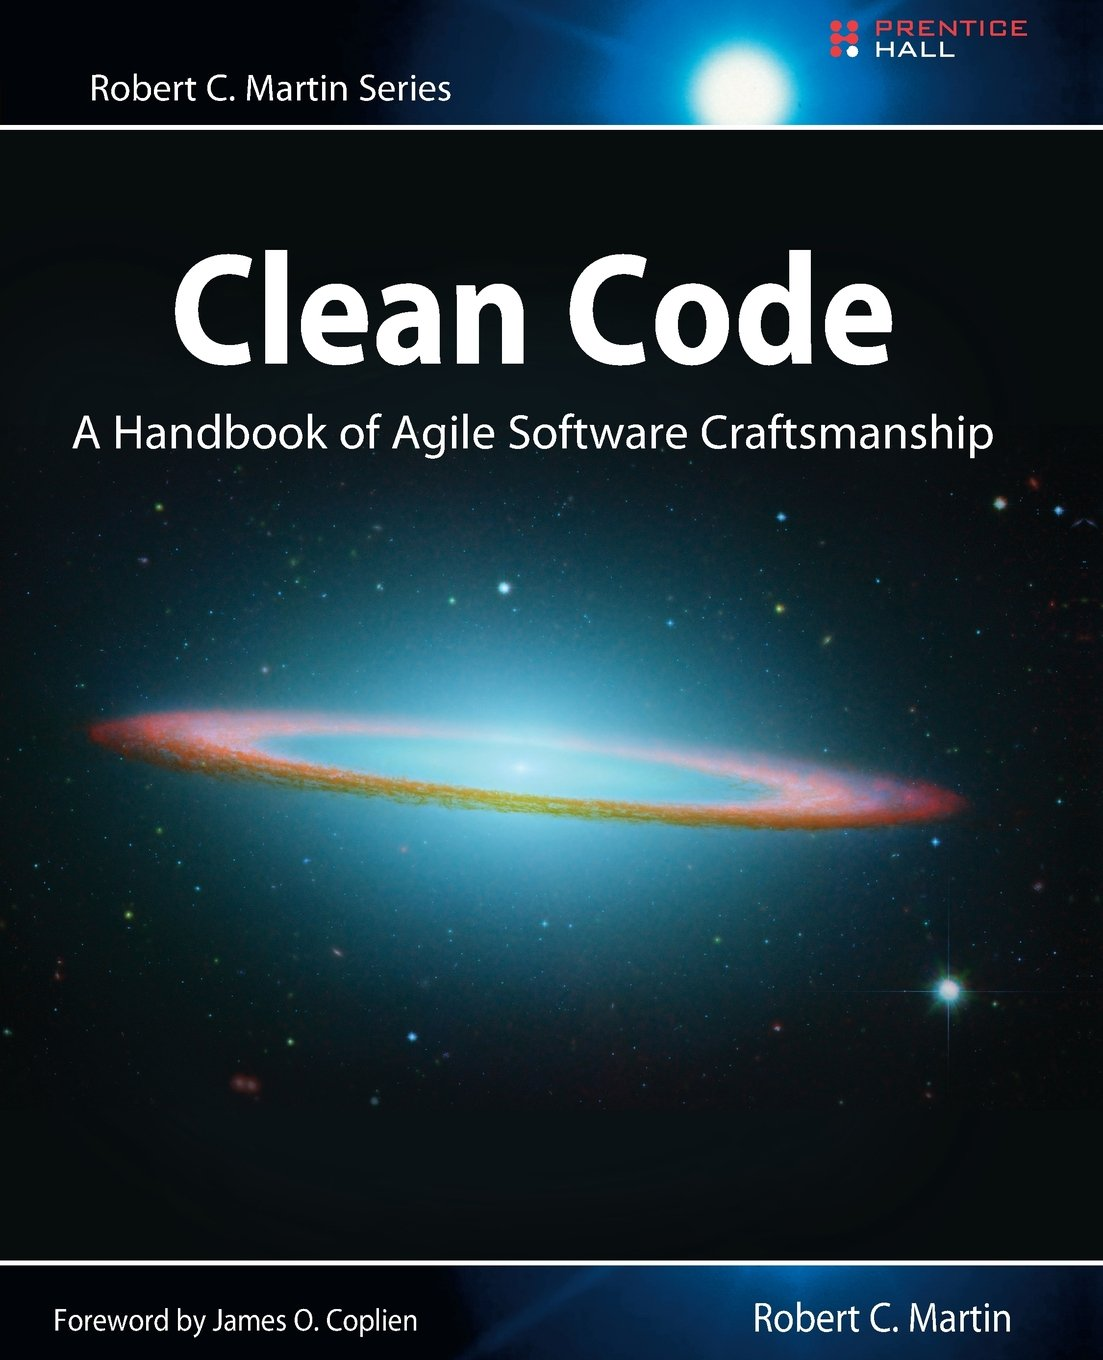
\includegraphics[height=35mm]{CleanCode.jpg}};
        \PrepareURLsymbol[PP]
        \node[below = 1mm of fig, font=\scriptsize, xshift=-2pt] {\URL*{http://clean-code-developer.com/}{The Clean Code developer road}};
        \node[below = 6mm of fig, font=\tiny] (progress) {
            %\href{http://clean-code-developer.com/grades/grade-0-black/}{Black} $\,\to\,$
            \PrepareURLsymbol[PQ]
            \URL*{http://clean-code-developer.com/grades/grade-1-red/}{Red} $\,\to\,$
            \PrepareURLsymbol[PT]
            \URL*{http://clean-code-developer.com/grades/grade-2-orange/}{Orange} $\,\to\,$
            \PrepareURLsymbol[Goldenrod]
            \URL*{http://clean-code-developer.com/grades/grade-3-yellow/}{Yellow} $\,\to\,$
            \PrepareURLsymbol[PS]
            \URL*{http://clean-code-developer.com/grades/grade-4-green/}{Green} $\,\to\,$
            \PrepareURLsymbol[PB]
            \URL*{http://clean-code-developer.com/grades/grade-5-blue/}{Blue} $\,\to\,$
            \PrepareURLsymbol[white]
            \colorbox{PP}{\URL*{http://clean-code-developer.com/grades/grade-6-white/}{White}}
        };
        \path[to] (progress.359) edge[out=350, in=190, looseness=1.2] (progress.181);
    \end{tikzpicture}
\end{frame}
%~~~~~~~~~~~~~~~~~~~~~~~~~~~~~~~~~~~~~~~~~~~~%
\begin{frame}{Why do we need to care?}
    \vspace{-8mm}
    \begin{overlayarea}{\textwidth}{0.8\textheight}
        \begin{onlyenv}<1>
            \begin{center}
                \vspace{3mm}
\includegraphics[width=0.6\textwidth]{Readability.jpg}
            \end{center}
        \end{onlyenv}
        \begin{uncoverenv}<3->
            \begin{quoteblock}{The technical debt}[Wikipedia]
                It is a concept that reflects the implied cost of additional rework caused
                by choosing an easy solution now instead of using a better approach that would take longer.\\[-1ex]
            \end{quoteblock}
        \end{uncoverenv}
        \begin{onlyenv}<2-3>
            \begin{itemize}
                \item We never write code for one \alert{time-invariant} reader!
                \item Learning and applying \PP{few simple rules} increases quality of code base.
                \item When a program is modified, its complexity will increase, provided that one does not actively work against this.
            \end{itemize}
        \end{onlyenv}
        \vspace{-8mm}
        \begin{onlyenv}<4->
            \begin{center}
                \begin{tikzpicture}[font=\footnotesize, node distance=9mm]
                    \coordinate (O) at (0,0);
                    \begin{scope}[scope on=<4->]
                        \node[thick, ellipse, Shape={PB}{PB!20}{PB}, text width=19mm, align=center, left  = of O] (A) {Quick and dirty implementation};
                        \node[thick, ellipse, Shape={PP}{PP!20}{PP}, text width=18mm, align=center, above = of O] (B) {Technical debt increases};
                        \path[to] (A) edge[out=90, in=180] (B);
                    \end{scope}
                    \begin{scope}[scope on=<4-5>]
                        \node[thick, ellipse, Shape={PT}{PT!20}{PT}, text width=18mm, align=center, below = of O] (C) {Harder to add new features};
                        \path[to] (B) edge[out=0, in=0, looseness=1.26] (C) (C) edge[out=180, in=270] (A);
                    \end{scope}
                    %\begin{scope}[scope on=<5>]
                    %    \node[starburst, starburst point height=15mm, minimum width=7cm, minimum height=5cm, Shape={red}{yellow!50}{red}, line width=1.5pt, font=\Huge\ttfamily, rotate=10] at (O) {BOOM};
                    %\end{scope}
                    \begin{scope}[scope on=<5>]
                       \node (VC) at ([yshift=-3mm]O) {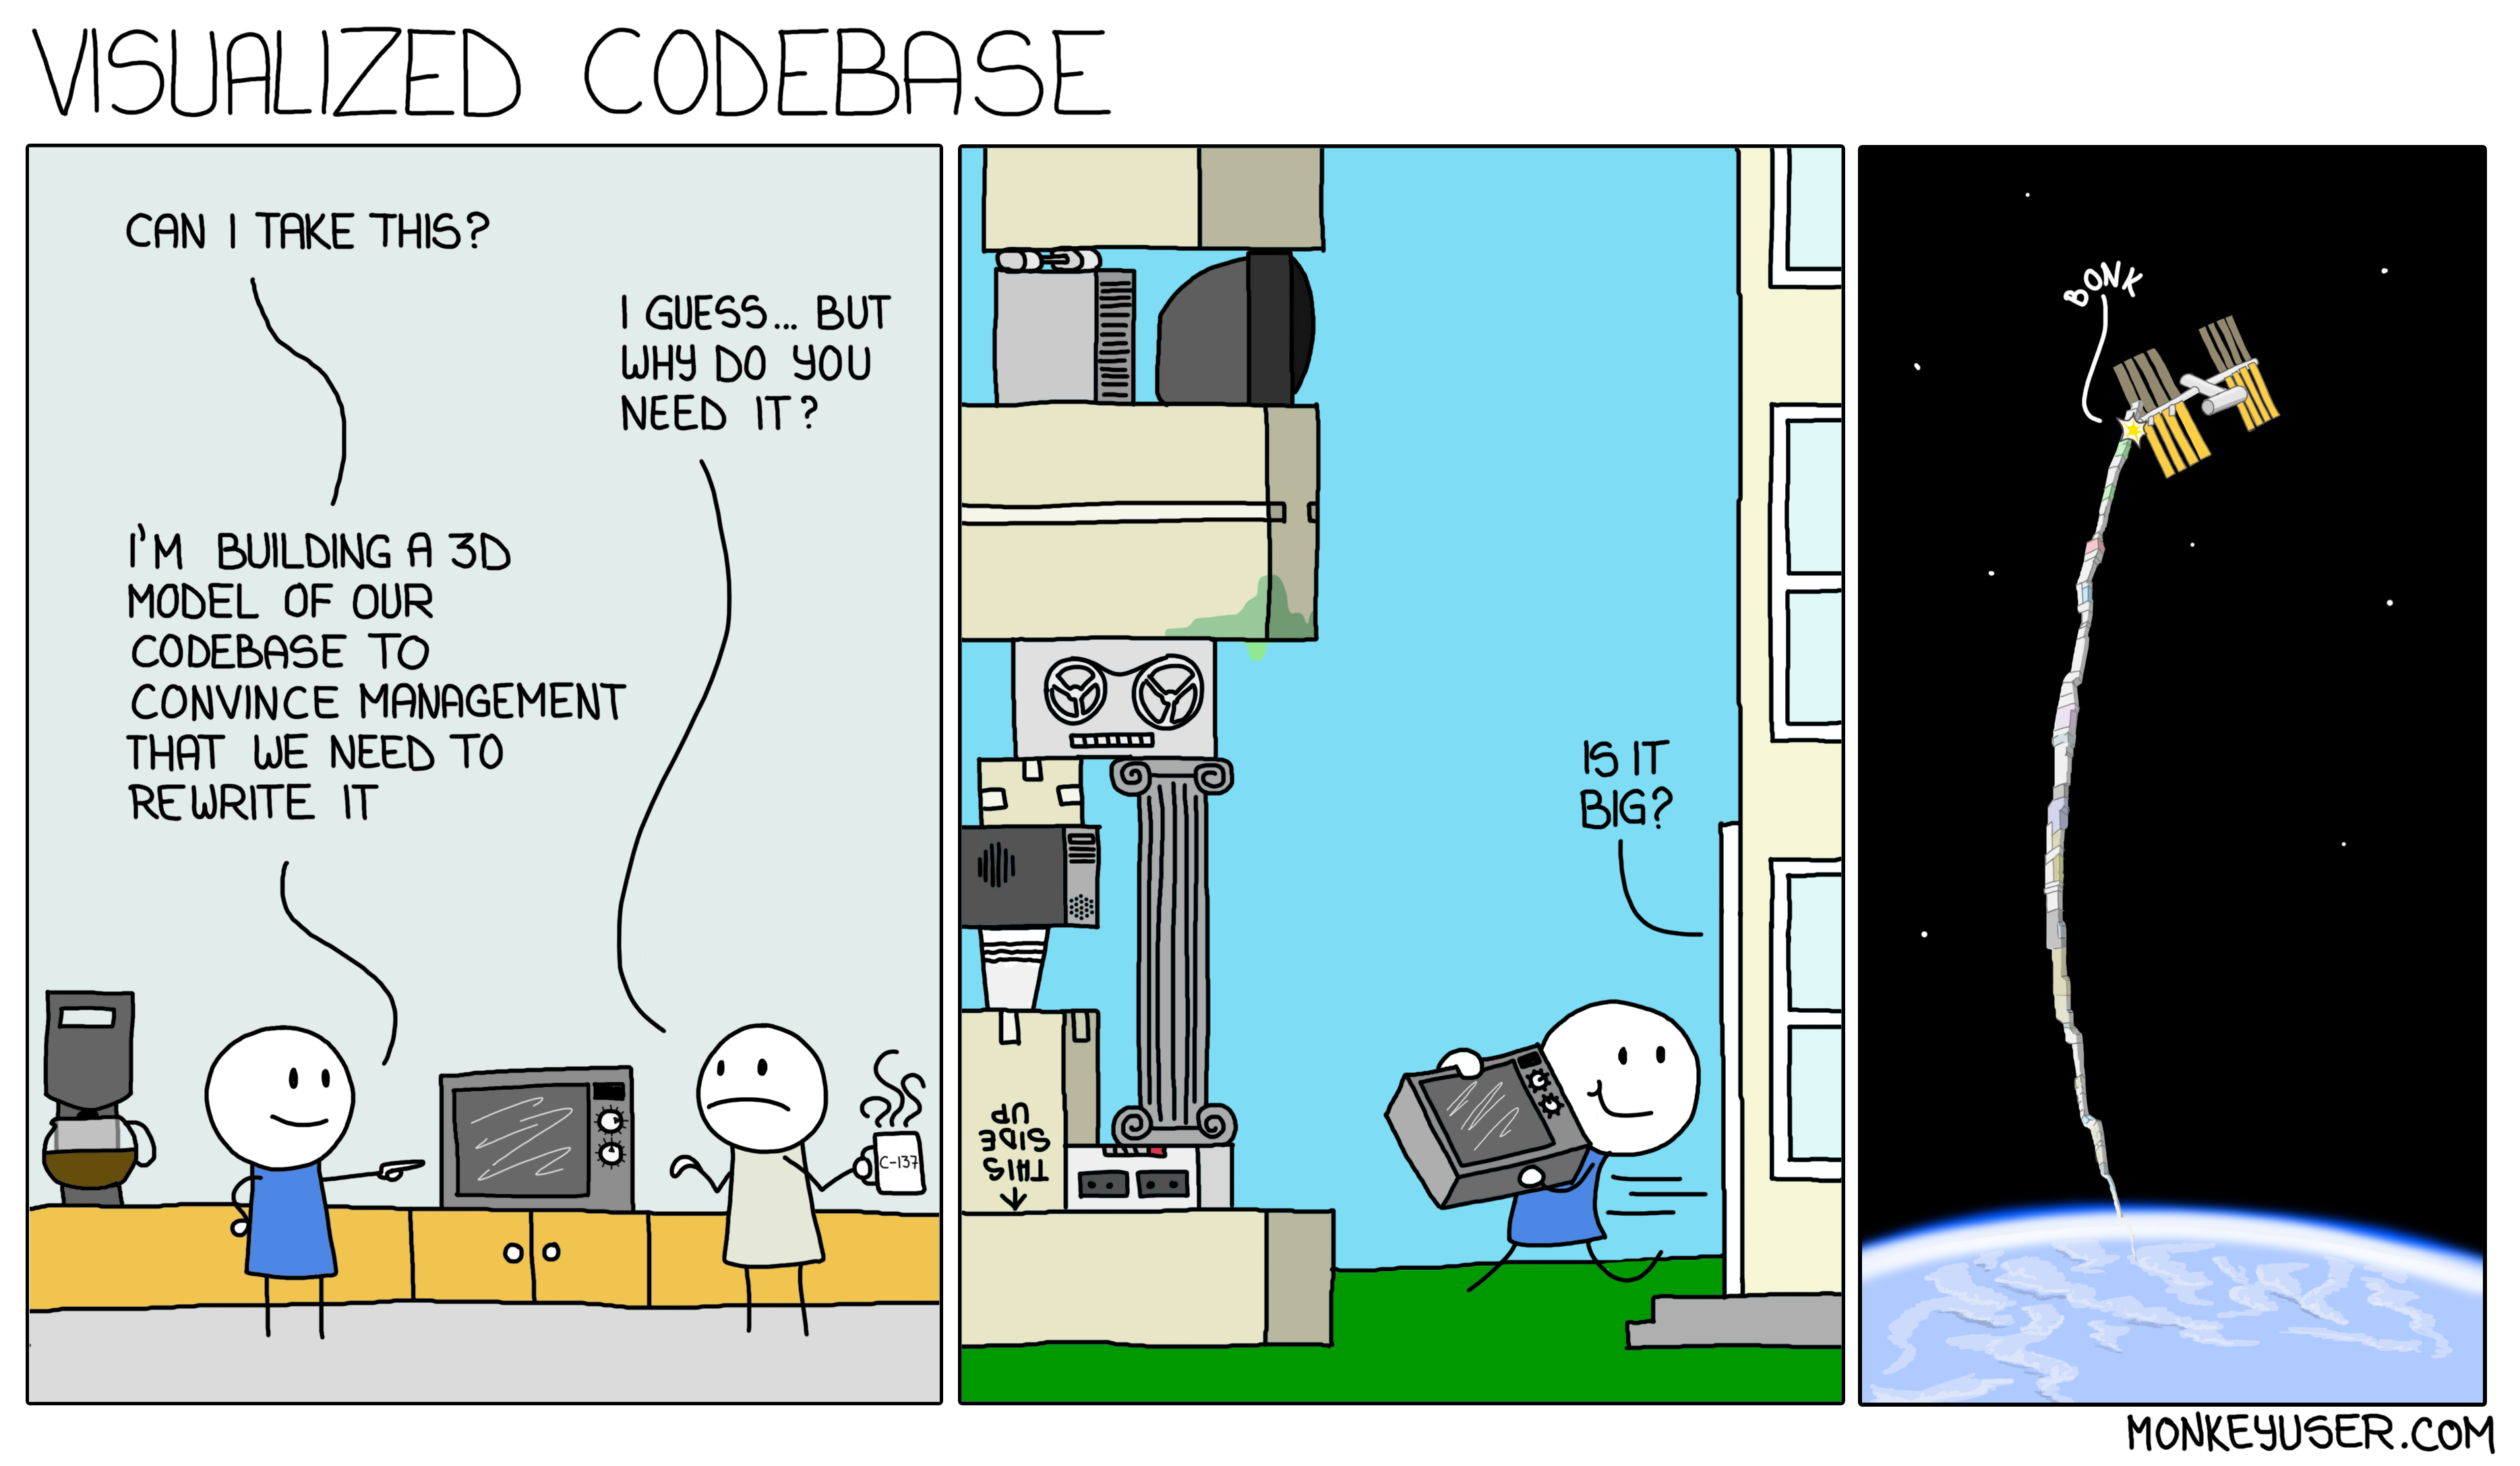
\includegraphics[height=0.6\textheight]{VisualizedCodebase}};
                       %\fill[white, visible on=<5>] ($(VC.south west)!0.76!(VC.south)+(0,3.8mm)$) rectangle ($(VC.north east)!0.21!(VC.east)-(2mm,0)$);
                    \end{scope}
                    \begin{scope}[scope on=<6->]
                        \node[thick, ellipse, Shape={PS}{PS!20}{PS}, text width=18mm, align=center, right = of O] (D) {Pay back technical debt};
                        \path[to] (B) edge[out=0, in=102] (D.86) (D.274) edge[out=265, in=270, looseness=0.6] (A);
                        \node[hexagon={red}{yellow!20}{red}, font=\small] (note) at ([yshift=-6mm]C) {Technical debt naturally tends to increase};
                        %\node[below = -1pt of note, font=\itshape\tiny, text=PB] {(in codebases which make use of external libraries)};
                    \end{scope}
                \end{tikzpicture}
            \end{center}
        \end{onlyenv}
    \end{overlayarea}
\end{frame}
%~~~~~~~~~~~~~~~~~~~~~~~~~~~~~~~~~~~~~~~~~~~~%
\begin{frame}{The connection to physics}{As physicist, why should I care of having high quality code?}
    \vspace{-3mm}
    \begin{itemize}
        \item It is plenty of problems which need to be approached numerically\\
              $\quad\to\;$ Programming is one of the major tasks in physics!
        \item Reproducibility should be a pillar of science\\
              $\quad\to\;$ One of the main responsibilities of a scientist!
        \item Lots of bad code around and passed on across generations\\
              $\quad\to\;$ A \PP{huge amount of time} is wasted, \PP{subtracted to research!}
    \end{itemize}
    \vspace{-2mm}
    \begin{varblock}{}{It should not happen\ldots}
        \guillemotleft{}Wow! There is definitely \alert{a new physics signal} in these data!\guillemotright\\
        {\color{PP}\scriptsize\ldots{}few days/weeks/months/years later\ldots}\\[0.5ex]
        \guillemotleft{}Oh, no! It was \alert{just a bug} in the code!\guillemotright
    \end{varblock}
\end{frame}
%~~~~~~~~~~~~~~~~~~~~~~~~~~~~~~~~~~~~~~~~~~~~%
\begin{frame}[c]{The starting point\ldots}
    \uncover<2>{\centerline{
\includegraphics[width=0.7\textwidth]{ButItRuns}}}
\end{frame}
%===================================================================================================%


%===================================================================================================%
\section{Meaningful names}
%~~~~~~~~~~~~~~~~~~~~~~~~~~~~~~~~~~~~~~~~~~~~%
\begin{frame}[fragile]{Use intention-revealing names}
    \vspace{-4mm}
    \begin{varblock}{block example}{\alt<1-2>{Why is it hard to tell what this code is doing?}{Good names are crucial for readability!}}
        \begin{onlyenv}<1-2>
            \begin{Cpp}[gobble=16]
                typedef std::vector< std::vector<int> > myVecVec;

                myVecVec FC(const myVecVec& b)
                {
                    myVecVec list;
                    for(const std::vector<int>& c : b){
                        if(c[0] == 4)
                            list.push_back(c);
                    }
                    return list;
                }
            \end{Cpp}
        \end{onlyenv}
        \begin{onlyenv}<3>
            \begin{Cpp}[gobble=16]
                typedef std::vector< std::vector<int> > myVecVec;

                myVecVec getFlaggedCells(const myVecVec& gameBoard)
                {
                    myVecVec flaggedCells;
                    for(const std::vector<int>& cell : gameBoard){
                        if(cell[STATUS_VALUE] == FLAGGED)
                            flaggedCells.push_back(cell);
                    }
                    return flaggedCells;
                }
            \end{Cpp}
        \end{onlyenv}
        \begin{onlyenv}<4>
            \begin{Cpp}[gobble=16]
                //typedef std::vector< std::vector<int> > myVecVec;

                SetOfCells getFlaggedCells(const SetOfCells& gameBoard)
                {
                    SetOfCells flaggedCells;
                    for(const Cell& cell : gameBoard){
                        if(cell.isFlagged())
                            flaggedCells.push_back(cell);
                    }
                    return flaggedCells;
                }
            \end{Cpp}
        \end{onlyenv}

    \end{varblock}
    \begin{uncoverenv}<2->
        \begin{itemize}
            \item What kind of object is contained in \alt<2>{\CPP|list|}{\CPP|flaggedCells|}?
            \item What does \alt<2>{\PB{0}}{\CPP|STATUS_VALUE|} represent in the \CPP|if|-clause?
            \item What does \alt<2>{\PB{4}}{\CPP|FLAGGED|} mean in the \CPP|if|-clause?
            \item How would I use the object being returned?
        \end{itemize}
    \end{uncoverenv}
\end{frame}
%~~~~~~~~~~~~~~~~~~~~~~~~~~~~~~~~~~~~~~~~~~~~%
\begin{frame}[fragile]{Use names which can be searched}
    \vspace{-9mm}
    \begin{overlayarea}{\textwidth}{\textheight}
        \begin{varblock}{}{Rule of thumb}
            The length of a name should correspond to the size of its scope
        \end{varblock}
        \vspace{-3mm}
        \begin{itemize}
            \item Single-letter names \alert{only} for local variables inside \alert{short scopes}
            \item IDE very good at renaming variables $\;\Rightarrow\;$ rename, rename, rename!
        \end{itemize}
        \vspace{-3mm}
        \begin{varblock}{block example}{Something like this\ldots}<only@2>
            \begin{Cpp}[gobble=16]
                for(int j = 0; j < 34; j++)
                    s += t[j]*4/5;
            \end{Cpp}
        \end{varblock}
        \begin{varblock}{block example}[\textwidth]{\ldots{}or something like this?}<only@3>
            \begin{Cpp}[gobble=16]
                const int realDaysPerIdealWeek = 4;
                int totalRealWeeksNeeded = 0;
                for(int j = 0; j < NUMBER_OF_TASKS; j++)
                {
                    int realDaysPerTask   = taskDaysEstimate.at(j) *
                                            realDaysPerIdealWeek;
                    int realWeeksPerTask  = realDaysPerTask/WORKING_DAYS_PER_WEEK;
                    totalRealWeeksNeeded += realWeeksPerTask;
                }
            \end{Cpp}
        \end{varblock}
    \end{overlayarea}
\end{frame}
%~~~~~~~~~~~~~~~~~~~~~~~~~~~~~~~~~~~~~~~~~~~~%
\begin{frame}[fragile]{Other important principles}
    \vspace{-3mm}
    \begin{itemize}
        \setlength{\itemindent}{-3mm}
        \item Avoid disinformation
        \item \alert{Use pronounceable names} $\;\to\;$ \PS{\texttt{timestamp}} better than \PQ{\texttt{ymdhms}}
        \item Avoid mental mapping
        \item Pick \alert{one} word per concept $\;\to\;$\CPP|get|, \CPP|fetch|, \CPP|retrieve|, \CPP|obtain|
        \item Do not be cute
        \item \ldots
    \end{itemize}
    \vspace{-3mm}
    \begin{varblock}{}[0.5\textwidth]{Take home lesson}
        \alert{Choose carefully} every name!
    \end{varblock}
    \vspace{-2mm}
    \begin{varblock}{}[0.5\textwidth]{}
        \alert{Rename} when you find better ones!
    \end{varblock}
\end{frame}
%===================================================================================================%


%===================================================================================================%
\section{Comments and Formatting}
%~~~~~~~~~~~~~~~~~~~~~~~~~~~~~~~~~~~~~~~~~~~~%
\begin{frame}{Do not comment bad code, rewrite it}
    \vspace{-3mm}
    \begin{quoteblock}{Avoid comments!}[R. C. Martin]
        The proper use of comments is to compensate for our failure to express ourself in code.
        Note that I used the word \alert{failure}. I meant it. Comments are always failures. [\ldots]
        Why am I so down on comments? Because they lie. Not always, and not intentionally, but too often.
        The older a comment is, and the farther away it is from the code it describes, the more likely
        it is to be just plain wrong.
    \end{quoteblock}
    \begin{itemize}
        \item To keep comments up-to-date costs energy and this energy should rather go into make the code clearer and more expressive!
        \item Inaccurate comments are far worse than no comments!
        \item Truth can only be found in one place: the code.
    \end{itemize}
\end{frame}
%~~~~~~~~~~~~~~~~~~~~~~~~~~~~~~~~~~~~~~~~~~~~%
\begin{frame}[fragile]{Explain yourself in the code}
    \vspace{-5mm}
    \begin{varblock}{block example}[0.85\textwidth]{What you should strive to avoid\ldots}
        \begin{Cpp}[gobble=12]
            Person e; // The employee we are considering

            // Check if the employee is eligible for full benefits
            if( (e.flags & HOURLY_FLAG) && e.age > 65 )
        \end{Cpp}
    \end{varblock}
    \begin{varblock}{block example}[0.8\textwidth]{\ldots{}in favour of expressive code}<2->
        \begin{Cpp}[gobble=12]
            Person employee;

            if(employee.isEligibleForFullBenefits())
        \end{Cpp}
    \end{varblock}
    \begin{uncoverenv}<3>
        \begin{itemize}
            \item It is simple to come up with good ideas
            \item It is often simply matter of creating a function whose name expresses the content of the comment!
        \end{itemize}
    \end{uncoverenv}
\end{frame}
%~~~~~~~~~~~~~~~~~~~~~~~~~~~~~~~~~~~~~~~~~~~~%
\begin{frame}[fragile]{Good comments}{But try to limit them as much as possible!}
    \vspace{-1mm}
    \begin{overlayarea}{\textwidth}{\textheight}
        \begin{onlyenv}<4->
            \begin{itemize}
                \item Informative comment
                \item Explanation of intent, Clarification
                \only<5->{\item Amplification}
                \only<6->{\item \PQ{TODO comments}{$\;$\scriptsize $\to\;$border line: really needed in a code? Take time to go through them!}}
                \only<6->{\item \PQ{Legal comments}{$\;$\scriptsize $\to\;$border line: not legally required \& overlap with version control.}}
            \end{itemize}
            \begin{onlyenv}<6->
                \begin{tikzpicture}[remember picture, overlay]
                    \node[anchor=north east] (TD) at ($(current page.north east)-(7mm,3mm)$) {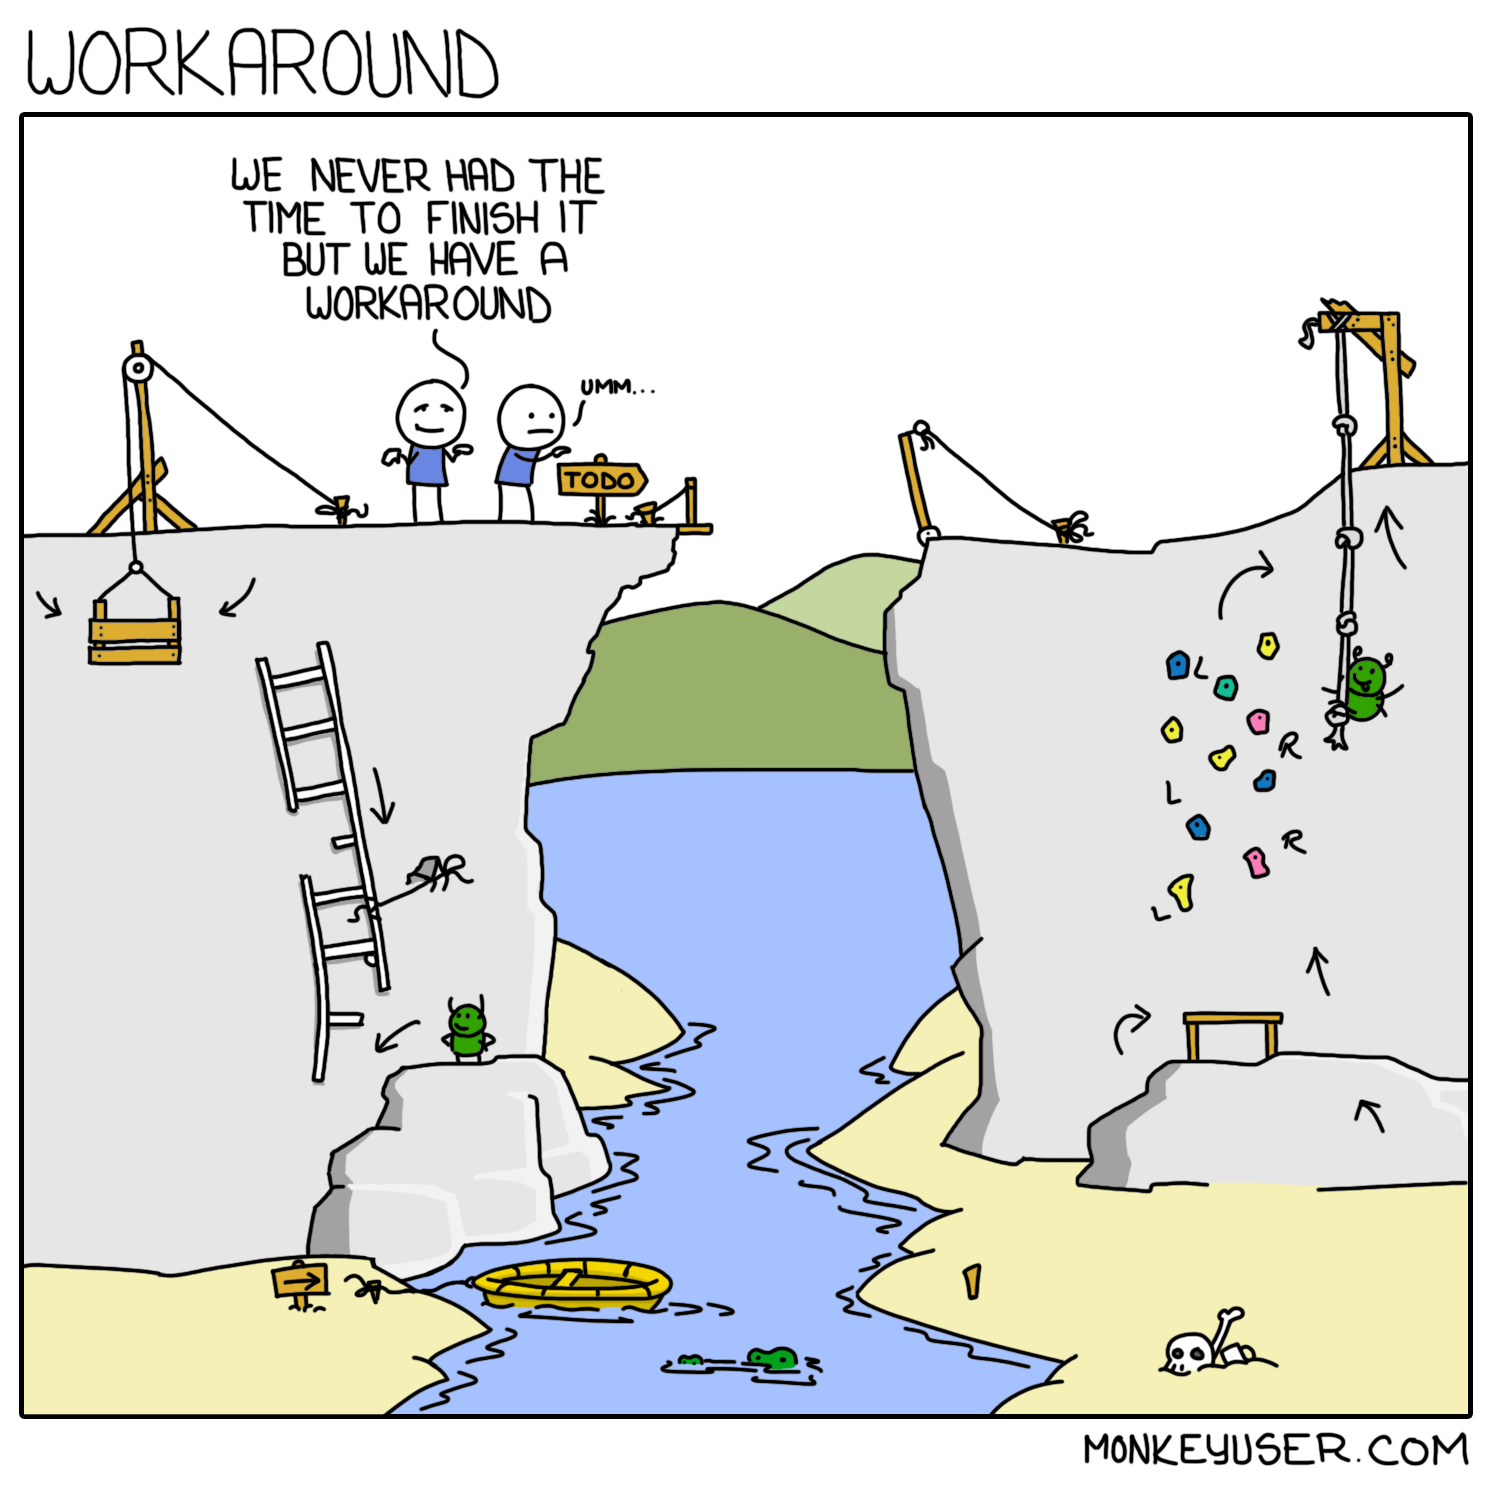
\includegraphics[scale=0.07]{Todo}};
                    \path[thin, to] ($(TD.south)!0.5!(TD.south east)$) edge[out=270, in=0] ++(-6.5mm,-4.8mm);
                \end{tikzpicture}
            \end{onlyenv}
        \end{onlyenv}
        \begin{onlyenv}<1-3>
            \vspace{-5mm}
            \begin{varblock}{block example}[0.98\textwidth]{Informative comment}
                \begin{Cpp}[gobble=20]
                    // Format matched:     hh:mm:ss dd Month yyyy
                    std::regex timePattern("(\\d{2}:){2}\\d{2}, \\d{2} \\S+ \\d{4}");
                \end{Cpp}
            \end{varblock}
            \begin{varblock}{block example}[0.77\textwidth]{Explanation of intent}<uncover@2->
                \begin{Cpp}[gobble=20]
                    // Checking the residuum possibly not every
                    // iteration allows for speed up on GPUs
                    if(iterationNumber % CG_CHECK_RESIDUUM_EVERY == 0)
                \end{Cpp}
            \end{varblock}
            \begin{varblock}{block example}[0.77\textwidth]{Clarification when using cryptic external API}<uncover@3>
                \begin{Cpp}[gobble=20]
                    // Check if root was found up to desired precision
                    if(gsl_fcmp(functionValue, 0.0, epsilon) == 0)
                \end{Cpp}
            \end{varblock}
        \end{onlyenv}
        \begin{varblock}{block example}[0.99\textwidth]{Amplification}<only@4>
            \begin{Cpp}[gobble=16]
                // See https://stackoverflow.com/a/1736040 for more information.
                template<typename T>
                std::string getDefaultForHelper(const T& number)
            \end{Cpp}
        \end{varblock}
        \vspace{-1mm}
        \begin{varblock}{block example}[0.99\textwidth]{}<only@4>
            \begin{Cpp}[gobble=16]
                // Removing trailing spaces is crucial since any would break the
                // following algorithm. It might leave the string unchanged, but
                // the absence of trailing spaces is at the moment not guaranteed!
                boost::trim_right(keyToDecipher);
            \end{Cpp}
        \end{varblock}
        \begin{onlyenv}<5>
            \begin{varblock}{block example}[0.98\textwidth]{TODO comments}
                \begin{Cpp}[gobble=20]
                    // TODO: The following two classes should be merged into one!
                \end{Cpp}
            \end{varblock}
            \vspace{-2mm}
            \begin{varblock}{block example}[0.7\textwidth]{Legal comments}
                \begin{Cpp}[gobble=20]
                    /*******************************************
                     *  Copyright (c) 2018 Alessandro Sciarra  *
                     *                                         *
                     *  This file is part of CL2QCD.           *
                     *******************************************/
                \end{Cpp}
            \end{varblock}
        \end{onlyenv}
        \vspace{-5mm}
        \begin{varblock}{block alerted}[0.96\textwidth]{Automatic documentation comments}<6>
            If you are writing a public API, then you should certainly provide a good documentation.
            But be aware that documentation comments can be as misleading, misplaced and lying as any other comment.
        \end{varblock}
    \end{overlayarea}
\end{frame}
%~~~~~~~~~~~~~~~~~~~~~~~~~~~~~~~~~~~~~~~~~~~~%
\begin{frame}[fragile]{Bad comments}
    \vspace{-5mm}
    \begin{overlayarea}{\textwidth}{\textheight}
        \begin{onlyenv}<1>
            \vspace{-4mm}
            \begin{varblock}{block example}[0.94\textwidth]{Several bad habits in one example}<only@1>
                \begin{Cpp}[gobble=20]
                    /**
                      * @param longTitle The complete title of the CD
                      * @param longAuthor The complete author of the CD
                      * @param nTracks The number of tracks of the CD
                      * @param durationInMinutes The duration of the CD in minutes
                      */
                    void Jukebox::addCD(std::string longTitle,
                                        std::string longAuthor,
                                        /*int nTracks,*/ int durationInMinutes)
                    {
                        // Create new CD to be later added to the list
                        CD cd;
                        cd.title    = longTitle;
                        cd.author   = longAuthor;
                        //cd.tracks   = nTracks;
                        cd.duration = durationInMinutes;
                        if(cd.duration<60) // Added by James
                            throw std::invalid_argument();
                        cdList.push_back(cd);
                    } // addCD method
                \end{Cpp}
            \end{varblock}
        \end{onlyenv}
        \begin{overlayarea}{\textwidth}{0.7\textheight}
            \begin{varblock}{block example}[0.7\textwidth]{The same code cleaned up}<only@2>
                \begin{Cpp}[gobble=20]
                    void Jukebox::addCD(std::string longTitle,
                                        std::string longAuthor,
                                        int durationInMinutes)
                    {
                        CD cd;
                        cd.title    = longTitle;
                        cd.author   = longAuthor;
                        cd.duration = durationInMinutes;
                        if(cd.duration<60)
                            throw std::invalid_argument();
                        cdList.push_back(cd);
                    }
                \end{Cpp}
            \end{varblock}
            \begin{onlyenv}<3>
                \begin{itemize}
                    \item Redundant comments               \hfill\makebox[55mm][l]{\PP{$\;\to\;$}\alert{Avoid}}
                    \item Noise comments                   \hfill\makebox[55mm][l]{\PP{$\;\to\;$}\alert{Avoid}}
                    \item Misleading comments              \hfill\makebox[55mm][l]{\PP{$\;\to\;$}\alert{Avoid}}
                    \item Comments instead of a good name  \hfill\makebox[55mm][l]{\PP{$\;\to\;$}\alert{Use good name}}
                    \item Closing brace comments           \hfill\makebox[55mm][l]{\PP{$\;\to\;$}\alert{Rarely}}
                    \item Attribution comments             \hfill\makebox[55mm][l]{\PP{$\;\to\;$}\alert{Delete, use version control}}
                    \item Commented-out code               \hfill\makebox[55mm][l]{\PP{$\;\to\;$}\alert{Delete, use version control}}
                    \item Unclear, cryptic comments        \hfill\makebox[55mm][l]{\PP{$\;\to\;$}\alert{Remove or clarify}}
                \end{itemize}
            \end{onlyenv}
        \end{overlayarea}
            \begin{varblock}{}[0.8\textwidth]{}<2->
                Have \PB{good reasons} (are they!?) before adding a comment!
            \end{varblock}
    \end{overlayarea}
\end{frame}
%~~~~~~~~~~~~~~~~~~~~~~~~~~~~~~~~~~~~~~~~~~~~%
\begin{frame}{Formatting}{Yes, formatting is important!}
    \vspace{-3mm}
    \begin{itemize}
        \item How big should be a file? \\ $\to\;$ Try to stay \PP{below few hundreds}, the reader will be grateful!
        \item Give some vertical breath to your code
        \item Care about length of lines (\PP{80} to \alert{140} characters) \\
              $\to\;$ Crucial if the code is readable from browser (e.g. \PP{GitHub})
        \item Consider horizontal alignment and spacing (e.g. \PP{around operators})
        \item Be coherent (e.g. \PP{braces})
        \item How to work when different people write in the same code base?
    \end{itemize}
    \vspace{-2mm}
    \begin{varblock}{block alerted}[0.6\textwidth]{E.g. clang-format}
        Agree on a style and \alert{use a tool} to enforce it
    \end{varblock}
\end{frame}
%===================================================================================================%


%===================================================================================================%
\section{Functions and Classes}
%~~~~~~~~~~~~~~~~~~~~~~~~~~~~~~~~~~~~~~~~~~~~%
\begin{frame}[fragile]{Common general aspects}
    \vspace{-8mm}
    \begin{overlayarea}{\textwidth}{\textheight}
        \begin{varblock}{block alerted}[0.5\textwidth]{SMALL}
            Do \alert{one} thing. Do it \alert{well}. Do it \alert{only}!
        \end{varblock}
        \begin{itemize}
            \item Functions and classes interfaces should stay small (fit one screen)
            \item \tc<2>{PP}{Classes should fulfil the single responsibility principle}
            \item \tc<3>{PP}{One level of abstraction per function}
        \end{itemize}
        \vspace{-2mm}
        \begin{varblock}{block example}[0.51\textwidth]{Single-responsibility class}<only@2>
            \begin{Cpp}[gobble=16]
                class Version {
                  public:
                    int getMajorVersionNumber();
                    int getMinorVersionNumber();
                    int getBuildNumber();
                };
            \end{Cpp}
        \end{varblock}
        \begin{varblock}{block example}[0.71\textwidth]{Single-level-of-abstraction function}<only@3>
            \begin{Cpp}[gobble=16]
                void MakeCoffee(const Coffee& typeOfCoffee){
                    WarmUpMachineIfNeeded(typeOfCoffee);
                    GrindCoffee(typeOfCoffee);
                    SetPressureAndTemperature(typeOfCoffee);
                    BrewCoffee(typeOfCoffee);
                }
            \end{Cpp}
        \end{varblock}
    \end{overlayarea}
\end{frame}
%~~~~~~~~~~~~~~~~~~~~~~~~~~~~~~~~~~~~~~~~~~~~%
\begin{frame}[fragile]{Limit the number of arguments}{Make useful abstractions whenever it helps}
    \vspace{-3mm}
    \begin{varblock}{block example}[\textwidth]{When you call the function, which argument is what?}
        \begin{Cpp}[gobble=12]
            double Distance(double, double, double, double);
            double Distance(double, double, double, double, double, double);
        \end{Cpp}
    \end{varblock}
    \begin{tikzpicture}
        \path coordinate (A) at (0,0) coordinate (B) at (3,1);
        \fill[PB] (A) circle[radius=1mm]; \fill[PB] (B) circle[radius=1mm];
        \draw[<->, >=stealth, shorten <= 4pt, shorten >= 4pt] (A) -- (B);
        \node[left = 2mm of A] {$A$};
        \node[right = 2mm of B] {$B$};
    \end{tikzpicture}
    \vspace{-1mm}
    \begin{varblock}{block example}[0.72\textwidth]{Isn't this much better?}<uncover@2>
        \begin{Cpp}[gobble=12]
            struct Point2D {      |    struct Point3D {
                double x, y;      |        double x, y, z;
            };                    |    };

            double Distance(std::pair<Point2D, Point2D>);
            double Distance(std::pair<Point3D, Point3D>);
        \end{Cpp}
    \end{varblock}
\end{frame}
%~~~~~~~~~~~~~~~~~~~~~~~~~~~~~~~~~~~~~~~~~~~~%
\begin{frame}[fragile]{\PQ{I}ntegration \PQ{O}peration \PQ{S}egregation \PQ{P}rinciple}
    \vspace{-9mm}
    \begin{overlayarea}{\textwidth}{\textheight}
        \begin{varblock}{block alerted}[\textwidth]{Clear separation of:}
            \begin{description}
                \item[Operation:]   A function which contains exclusively logic, meaning transformations, control structures or API invocations.
                \item[Integration:] A function which does not contain any logic but exclusively calls other functions of the code base.
            \end{description}
        \end{varblock}
        \vspace{-1mm}
        \begin{varblock}{block example}[0.78\textwidth]{Operation}<only@1>
            \begin{Cpp}[gobble=16]
                bool isPrime(unsigned int number)
                {
                    if(number == 1) return false;
                    for(unsigned int i = 2; i <= sqrt(number); ++i)
                    {
                        if(number%i == 0) return false;
                    }
                    return true;
                }
            \end{Cpp}
        \end{varblock}
        \begin{varblock}{block example}[0.62\textwidth]{Integration}<only@2>
            \begin{Cpp}[gobble=16]
                int main(int argc, char *argv[])
                {
                    WelcomeUserToTheGame();
                    Minesweeper minesweeper(argc, argv);
                    minesweeper.playGame();
                    PrintGameResult();
                }
            \end{Cpp}
        \end{varblock}
    \end{overlayarea}
\end{frame}
%===================================================================================================%


%===================================================================================================%
\section{(Unit) Tests}
%~~~~~~~~~~~~~~~~~~~~~~~~~~~~~~~~~~~~~~~~~~~~%
\begin{frame}{Software testing}{Test code is just as important as production code}
    \vspace{2mm}
    \begin{columns}[c]
        \begin{column}{0.5\textwidth}
            \begin{itemize}
                \item \PP{Testing levels}
                      \begin{itemize}
                          \item \alert<2>{Unit testing}
                          \item \tc<2>{PQ}{Integration testing}
                          \item System testing
                          \item Acceptance testing
                      \end{itemize}
                \item \PP{Testing types and techniques}
                      \begin{itemize}
                          \item \alert<2>{Regression testing}
                          \item \alert<2>{Automated testing}
                          \item Continuous testing
                          \item \ldots
                      \end{itemize}
            \end{itemize}
        \end{column}
        \begin{column}{0.5\textwidth}
            \centering
            \begin{uncoverenv}<2>
                
\includegraphics[height=32mm]{SoftwareTesting.jpeg}$\quad$
                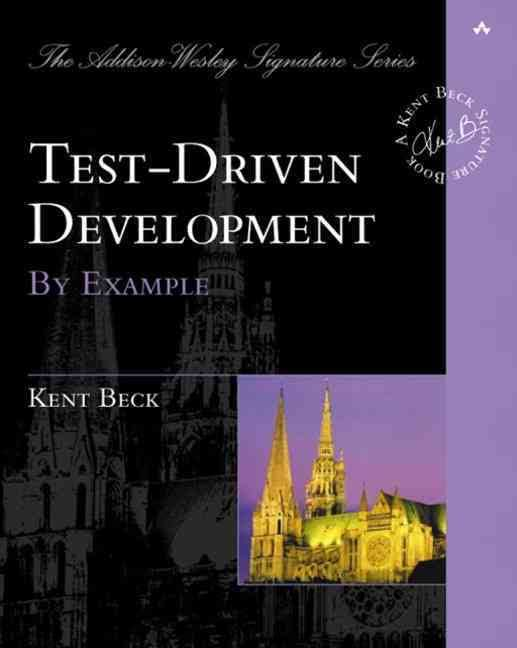
\includegraphics[height=32mm]{TDD.jpeg}
            \end{uncoverenv}
        \end{column}
    \end{columns}

\end{frame}
%~~~~~~~~~~~~~~~~~~~~~~~~~~~~~~~~~~~~~~~~~~~~%
\begin{frame}{The \PQ{wrong} mental approach to testing}
    \vspace{-2mm}
    \begin{itemize}
        \item I do not have time to waste writing tests.
        \item \alert{The result is reasonable, the code should be correct!}
        \item This part of code is simple, why should I test it?
        \item Let me finish to implement this feature so that I can produce some data and in the meanwhile I write some tests.
    \end{itemize}
    \begin{center}
        \begin{tikzpicture}
            \node (fig) {
\includegraphics[width=0.45\textwidth]{WrongTesting}};
            \node[anchor=north, font=\Tiny] at ([yshift=1mm]fig.south) {\url{https://android.jlelse.eu/basics-of-unit-testing-affdd2273310}};
            \draw[red, line width=2mm, visible on=<2>] (fig.south east) -- (fig.north west) (fig.south west) -- (fig.north east);
        \end{tikzpicture}
    \end{center}
    \begin{tikzpicture}[overlay, remember picture]
        \node[starburst, starburst points=27, starburst point height=16mm, minimum width=12cm, minimum height=5cm,
              Shape={red}{yellow!50}{red}, line width=1.5pt, font=\Huge, rotate=10, visible on=<2>] at ([shift={(-0mm,21mm)}]current page.center) {Please, NO!};
    \end{tikzpicture}
\end{frame}
%~~~~~~~~~~~~~~~~~~~~~~~~~~~~~~~~~~~~~~~~~~~~%
\begin{frame}{The \PS{correct} mental approach to testing}
    \begin{itemize}
        \setlength{\itemindent}{-2mm}
        \item Testing is part of the natural evolution of the code (not an overhead)
        \item Test code has to fulfil the same clean code rules as production code
        \item \alert{Tests are the key to be free to change (improve) the production code!}
        \item Keep balance between adding new code, writing tests and refactoring
    \end{itemize}
    \begin{uncoverenv}<2>
        \begin{center}
            \resizebox{!}{0.32\textheight}{
                \begin{tikzpicture}
                    \tikzstyle{Pie}=[font=\Large]
                    \tikzstyle{PieNum}=[font=\Large\bfseries\ttfamily]
                    \piechartthreed[scale=0.8, background color=white, mix color= white]{120/PS!50!LimeGreen,120/PP!50!white,120/PT}
                    \foreach \i in {1,...,3} { \fill (pc \i) ellipse (0.1 and 0.05);}
                    \draw[darkgray] (pc 1)  -- ++(7,0) coordinate (s1)              node[Pie, anchor=south east] {Testing}      node[PieNum, anchor=north east] {\tc{PS}{33\%}};
                    \draw[darkgray] (pc 2)  -- ++(-1,1) -- ++(-5,0) coordinate (s2) node[Pie, anchor=south west] {Developing}   node[PieNum, anchor=north west] {\tc{PP}{33\%}};
                    \draw[darkgray] (pc 3)  -- (pc 3 -| s2)                         node[Pie, anchor=south west] {Refactoring}  node[PieNum, anchor=north west] {\tc{PT}{33\%}};
                \end{tikzpicture}
            }
        \end{center}
    \end{uncoverenv}

\end{frame}
%~~~~~~~~~~~~~~~~~~~~~~~~~~~~~~~~~~~~~~~~~~~~%
\begin{frame}{The five principles clean tests should fulfil}
    \begin{center}
        \begin{minipage}{0.76\textwidth}
            \begin{description}[Self-validating:]
                \item[\PQ{F}ast:] To be run frequently
                \item[\PQ{I}ndependent:] To make failures meaningful
                \item[\PQ{R}epeatable:] To be run everywhere with same outcome
                \item[\PQ{S}elf-validating:] To be automatised
                \item[\PQ{T}imely:] To make production code testable
            \end{description}
        \end{minipage}
    \end{center}
    \begin{varblock}{block alerted}[0.6\textwidth]{Golden rule}
        \PQ{Write (or at least think) F.I.R.S.T. tests first!}
    \end{varblock}
\end{frame}
%~~~~~~~~~~~~~~~~~~~~~~~~~~~~~~~~~~~~~~~~~~~~%
\begin{frame}[fragile]{Unit tests}{The deeper level of testing}
    \vspace{-6.5mm}
    \begin{overlayarea}{\textwidth}{\textheight}
        \begin{varblock}{}[0.8\textwidth]{}
            \PB{Write tests for (every) unit of source code in the code base}
        \end{varblock}
        \begin{onlyenv}<1>
            \vspace{2mm}
            \begin{itemize}
                \item A \PP{unit}: the smallest testable part of a code (e.g. \PP{function/method})
                \item Strive to test a \PQ{single concept} per test function
                \item In most languages, \alert{unit tests frameworks} are available
                \item Automatic build tools (e.g. CMake) offers a natural way to run tests
                \item Know how much code you tested\\
                      $\;\to\;$ Code coverage tools (e.g. \URL[PP]{https://github.com/linux-test-project/lcov}{LCOV})
            \end{itemize}
        \end{onlyenv}
        \vspace{-2.5mm}
        \begin{varblock}{block example}[0.8\textwidth]{Boost unit test framework}<only@2>
            \begin{Cpp}[gobble=16]
                #define BOOST_TEST_MODULE Factorial
                #include |+<boost/test/included/unit_test.hpp>+|
                #include |+"factorial.hpp"+|

                BOOST_AUTO_TEST_CASE(SpecialCases)
                {
                    BOOST_REQUIRE_EQUAL(factorial(0), 1);
                    BOOST_REQUIRE_EQUAL(factorial(1), 1);
                }

                BOOST_AUTO_TEST_CASE(NormalCases)
                {
                    BOOST_REQUIRE_EQUAL(factorial(5), 120);
                }
            \end{Cpp}
        \end{varblock}
        \begin{varblock}{block example}[0.8\textwidth]{\small\texttt{./factorialTest\vphantom{p}}}<only@3>
            \begin{Cpp}[gobble=16]
                Running 2 test cases...
                boostTest.cpp(12): fatal error in "SpecialCases": critical check factorial(0) == 1 failed [0 != 1]

                *** 1 failure detected in test suite "Factorial"
            \end{Cpp}
        \end{varblock}
        \begin{varblock}{block example}[0.8\textwidth]{\small\texttt{./factorialTest --report\_level=short}}<only@4>
            \begin{Cpp}[gobble=16]
                Running 2 test cases...
                boostTest.cpp(12): fatal error in "SpecialCases": critical check factorial(0) == 1 failed [0 != 1]

                Test suite "Factorial" failed with:
                  1 assertion out of 2 passed
                  1 assertion out of 2 failed
                  1 test case out of 2 passed
                  1 test case out of 2 failed
                  1 test case out of 2 aborted
            \end{Cpp}
        \end{varblock}
        \begin{varblock}{block example}[0.8\textwidth]{\small\texttt{./factorialTest --report\_level=detailed}}<only@5>
            \begin{Cpp}[gobble=16]
                Running 2 test cases...
                boostTest.cpp(12): fatal error in "SpecialCases": critical check factorial(0) == 1 failed [0 != 1]

                Test suite "Factorial" failed with:
                  1 assertion out of 2 passed
                  1 assertion out of 2 failed
                  1 test case out of 2 passed
                  1 test case out of 2 failed
                  1 test case out of 2 aborted

                  Test case "SpecialCases" aborted with:
                    1 assertion out of 1 failed
                  Test case "NormalCases" passed with:
                    1 assertion out of 1 passed
            \end{Cpp}
        \end{varblock}
    \end{overlayarea}
    \begin{uncoverenv}<2->
        \PrepareURLsymbol[PB]
        \begin{tikzpicture}[remember picture, overlay]
            \node[anchor=north east, font=\footnotesize] at ([shift={(-6mm,-6mm)}]current page.north east)
                 {\URL*{https://www.boost.org/doc/libs/1_67_0/libs/test/doc/html/index.html}{Boost.Test} \PP{$\leftarrow$ Check me out!}};
        \end{tikzpicture}
    \end{uncoverenv}
\end{frame}
%~~~~~~~~~~~~~~~~~~~~~~~~~~~~~~~~~~~~~~~~~~~~%
\begin{frame}{What should I test and how?}
    \begin{itemize}
        \item Values \\ \uncover<2->{\centerline{
\includegraphics[scale=0.1]{TestingValue}}}
        \item Actions \\ \uncover<3->{\centerline{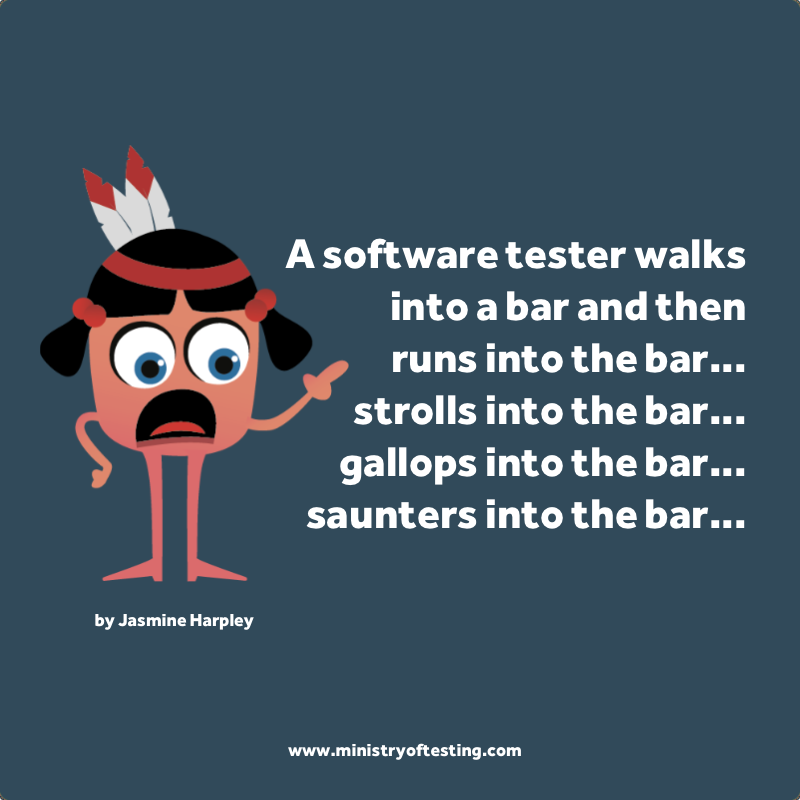
\includegraphics[scale=0.12, clip, trim=0 4cm 0 4cm]{TestingAction}}}
    \end{itemize}
    \uncover<3>{\hfill\ldots{}and anything that makes sense!}
\end{frame}
%~~~~~~~~~~~~~~~~~~~~~~~~~~~~~~~~~~~~~~~~~~~~%
\begin{frame}{Unit tests are not enough!}
    \begin{varblock}{}[0.9\textwidth]{Integration tests}
        \PB{Once you are sure that all components work correctly alone, be sure they work as expected together!}
    \end{varblock}
    \uncover<2>{
        \begin{center}
            
\includegraphics[height=4cm]{UnitTestVSIntegrationTestA}$\quad$
            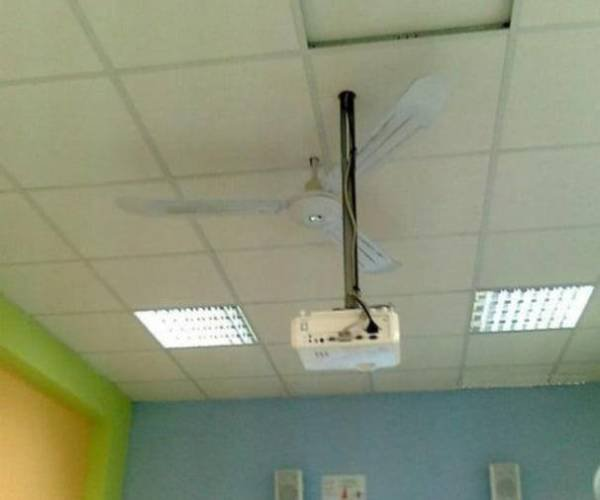
\includegraphics[height=4cm]{UnitTestVSIntegrationTestB}
        \end{center}
    }
\end{frame}
%===================================================================================================%


%===================================================================================================%
\section{General good practices}
%~~~~~~~~~~~~~~~~~~~~~~~~~~~~~~~~~~~~~~~~~~~~%
\begin{frame}[fragile]{\PQ{D}on't \PQ{R}epeat \PQ{Y}ourself}
    \vspace{-3mm}
    \begin{overlayarea}{\textwidth}{\textheight}
        \begin{itemize}
            \item If you are doing \alert{\emph{Copy \& Paste}}, you are doing it wrong!
            \item One of the most basic and yet most disregarded principle
            \item Code duplication makes the code less maintainable and easy to break
        \end{itemize}
        \begin{varblock}{block example}[11cm]{Trivial example}<only@2-3>
            \begin{onlyenv}<2>
                \begin{Cpp}[gobble=18]
                    double sum1=0;
                    for(const auto& data : dataSet1)
                        sum1 += data;
                    sum1 /= dataSet1.size();


                    double sum2=0;
                    for(const auto& data : dataSet2)
                        sum2 += data;
                    sum2 /= dataSet2.size();
                \end{Cpp}
            \end{onlyenv}
            \begin{onlyenv}<3>
                \begin{Cpp}[gobble=18]
                    double calculateAverage(const std::vector<double>& dataSet)
                    {
                        double sum=0;
                        for(const auto& data : dataSet)
                            sum += data;
                        return sum / dataSet.size();
                    }

                    calculateAverage(dataSet1);
                    calculateAverage(dataSet2);
                \end{Cpp}
            \end{onlyenv}
        \end{varblock}
        \begin{varblock}{block example}[0.98\textwidth]{Less trivial example}<4->
            \begin{Cpp}[gobble=16]
                double calculateAverage(const std::vector<double>& dataSet)
                {
                   std::cout << "Function \"calculateAverage\" missing!\n";
                   exit(-1);
                }
             \end{Cpp}
            \begin{uncoverenv}<5>
                \begin{Cpp}[gobble=20]
                    double calculateAverage(const std::vector<double>& dataSet)
                    {
                       std::cout << "Function \"" << __FUNCTION__ << "\" missing!\n";
                       exit(-1);
                    }
                \end{Cpp}
            \end{uncoverenv}
        \end{varblock}
    \end{overlayarea}
\end{frame}
%~~~~~~~~~~~~~~~~~~~~~~~~~~~~~~~~~~~~~~~~~~~~%
\begin{frame}[fragile]{\PQ{K}eep \PQ{I}t \PQ{S}imple, \PQ{S}tupid}
    \begin{overlayarea}{\textwidth}{\textheight}
        \vspace{-9mm}
        \begin{quoteblock}{Avoid complexity!}[A. Einstein]
            Everything should be done as simple as possible, but not simpler.
        \end{quoteblock}
        \begin{onlyenv}<1>
            \begin{itemize}
                \item If you have a solution, ask yourself if there is an easier one
                \item Complexity reduces readability and maintainability
                \item \alert{Use libraries!}
                \item Do not feel cool because you did something hard in a tricky way.\\ \PP{Feel cool when you did the same in a trivial-to-understand way!}
                \item If you really need something complicated (do you!?), then be sure everybody understands!
            \end{itemize}
        \end{onlyenv}
        \vspace{-5mm}
        \begin{varblock}{block example}[0.86\textwidth]{Simple example}<only@2-4>
            \begin{onlyenv}<2>
                \begin{Cpp}[gobble=20]
                    std::vector<int> data = {1, -3, 2 8, 4, -9};

                    auto first = data.begin(), last = data.end();
                    while (first != last) {
                        if (*first == 4) {
                            makeReportForUser();
                            break;
                        }
                        ++first;
                    }
                \end{Cpp}
            \end{onlyenv}
            \begin{onlyenv}<3>
                \begin{Cpp}[gobble=20]
                    std::vector<int> data = {1, -3, 2 8, 4, -9};

                    auto it = std::find(data.begin(), data.end(), 4);
                    if(it != data.end())
                        makeReportForUser();
                \end{Cpp}
            \end{onlyenv}
            \begin{onlyenv}<4>
                \begin{Cpp}[gobble=20]
                    std::vector<int> data = {1, -3, 2 8, 4, -9};

                    //Even better
                    if(isElementInVector(data, 4))
                        makeReportForUser();
                \end{Cpp}
            \end{onlyenv}
        \end{varblock}
        \begin{onlyenv}<4>
            \vspace{-1mm}
            \begin{varblock}{block example}[0.86\textwidth]{}
                \begin{Cpp}[gobble=20]
                    template<typename T>
                    bool isElementInVector(const std::vector<T>& data,
                                           const T& value)
                    {
                        auto it = std::find(data.begin(), data.end(), value);
                        return it != data.end();
                    }
                \end{Cpp}
            \end{varblock}
        \end{onlyenv}
        \begin{varblock}{block example}[0.88\textwidth]{Example from real life (Quake III Arena, 1999)}<only@5-6>
            \begin{uncoverenv}<6>
                \begin{Cpp}[gobble=20]
                    float Q_rsqrt(float number)
                    {
                        long i;  float x2, y;  const float threehalfs = 1.5F;

                        x2 = number * 0.5F;  y  = number;
                        // evil floating point bit level hacking
                        i  = * (long*) &y;
                        i  = 0x5f3759df - (i >> 1);  // what the fuck?
                        y  = * (float*) &i;
                        // 1st iteration
                        y  = y * (threehalfs - (x2 * y * y));
                        // 2nd iteration, this can be removed
                        // y  = y * (threehalfs - (x2 * y * y));
                        return y;
                    }
                \end{Cpp}
            \end{uncoverenv}
        \end{varblock}
        \begin{varblock}{block example}[0.78\textwidth]{Example from real life (Quake III Arena, 1999)}<only@7->
            \begin{Cpp}[gobble=16]
                float Q_fastInverseSqrt(float number)
                {
                    float approximateResult
                       = calculateApproximateInverseSqrt(number);
                    return refineResult(approximateResult, number);
                }
            \end{Cpp}
        \end{varblock}
        \vspace{-2mm}
        \begin{varblock}{block example}[0.9\textwidth]{}<only@8>
            \PrepareURLsymbol[red]
            \begin{Cpp}[gobble=16]
                float calculateApproximateInverseSqrt(float number)
                {
                    //Here some very low level operations are carried out.
                    //Read @|\URL*{https://en.wikipedia.org/wiki/Fast\_inverse\_square\_root\#Algorithm}{here}|@ for a detailed explanation.
                    long floatAsInteger = * (long*) &number;
                    floatAsInteger = 0x5f3759df - (floatAsInteger >> 1);
                    return * (float*) &i;
                }
            \end{Cpp}
        \end{varblock}
        \begin{varblock}{block example}[0.9\textwidth]{}<only@9>
            \begin{Cpp}[gobble=16]
                float refineResult(float result, float initialNumber)
                {
                    //Here one iteration of the Newton's method is used.
                    //Read @|\URL*{https://en.wikipedia.org/wiki/Fast\_inverse\_square\_root\#Newton's\_method}{here}|@ for a detailed explanation.
                    float refinedResult = initialNumber * result * result;
                    return (3.0F - refinedResult) * result * 0.5F;
                }
            \end{Cpp}
        \end{varblock}
    \end{overlayarea}
\end{frame}
%~~~~~~~~~~~~~~~~~~~~~~~~~~~~~~~~~~~~~~~~~~~~%
\begin{frame}{Beware of optimisations}
    \vspace{-5mm}
    \begin{quoteblock}{Premature optimisation}[D. Knuth]
        Programmers waste enormous amounts of time thinking about, or worrying about,
        the speed of noncritical parts of their programs, and these attempts at efficiency
        actually have a strong negative impact when debugging and maintenance are considered.
        We should forget about small efficiencies, say about 97\% of the time:
        \par\smallskip
        \centerline{\alert{\textbf{Premature optimisation is the root of all evil}.}}
        \par\smallskip
        Yet we should not pass up our opportunities in that critical 3\%.
    \end{quoteblock}
    \vspace{-3mm}
    \begin{itemize}
        \item Compiler do more and more a better job!
        \item Use optimisations flags (e.g. \PP{\texttt{-O1}}, \PP{\texttt{-O3}} with \texttt{g++} and \texttt{clang})
        \item \alert{Never} sacrifice clean code in name of claimed better performance!
        \item Only optimise after having used a profiler and having written tests!
    \end{itemize}
\end{frame}
%~~~~~~~~~~~~~~~~~~~~~~~~~~~~~~~~~~~~~~~~~~~~%
\begin{frame}{The pathfinder rule}
    \begin{columns}[c]
        \begin{column}{0.4\textwidth}
            \begin{varblock}{}[\columnwidth]{}
                \color{PB}Leave the campground cleaner than you found it
            \end{varblock}
        \end{column}
        \begin{column}{0.45\textwidth}
            
\includegraphics[width=0.9\textwidth]{Firecamp.jpg}
        \end{column}
    \end{columns}
    \vspace{3mm}
    \begin{itemize}
        \item To clean an existing code base takes time and requires effort
        \item Aim for tiny but continuous progress
        \item Applying the pathfinder rule is a natural way to pay back technical debt
        \item Any IDE will help you in quickly achieving easy refactoring
    \end{itemize}
\end{frame}
%===================================================================================================%


%===================================================================================================%
\section{What to do, now?}
%~~~~~~~~~~~~~~~~~~~~~~~~~~~~~~~~~~~~~~~~~~~~%
\againframe<2>{THM}
%~~~~~~~~~~~~~~~~~~~~~~~~~~~~~~~~~~~~~~~~~~~~%
\begin{frame}{Go back and immediately apply what you learnt!}{Keep in mind good practices next time you code}
    \begin{itemize}
        \item Use these slides as a starting point
        \item Try to apply principles day after day
        \item \alert{Feel guilty when you do something dirty}
        \item \PP{Never give up} in writing high quality code
        \item Refer to the literature and go beyond this material, keep improving
        \item Develop your \PP{code-sense}, experience will make you quicker
    \end{itemize}
    \begin{quoteblock}{Moral of the story}[R. C. Martin]
        An old violinist got lost on his way to a performance.
        He stopped an old man on the corner and asked him how to get to Carnegie Hall.
        The old man looked at the violinist and the violin tucked under his arm and said:
        \alert{\guillemotleft{}Practice, son. Practice!\guillemotright}
    \end{quoteblock}
    \begin{tikzpicture}[remember picture, overlay]
        \node[anchor=north east, cloud, aspect=2, draw=PB, fill=PP!20, text=PB, visible on=<2>] at ($(current page.north east)+(-14mm,-20mm)$) {Thank you!};
    \end{tikzpicture}
\end{frame}
%===================================================================================================%


\end{document}
